\documentclass{article}
\usepackage{graphicx, color}


\setlength{\textwidth}{6.5in}
\setlength{\textheight}{8.5in}
\setlength{\oddsidemargin}{0in}
\setlength{\evensidemargin}{0in}
\setlength{\parskip}{2ex}
\setlength{\parindent}{0in}

%To display answers, replace "white" with "red" here;
\newcommand{\answer}[1]{\color{red}#1}


\begin{document}
\pagestyle{myheadings}\markright{
CU Boulder \hspace{0.5in} MATH 2510 - Introduction to Statistics}

\begin{center}
\textbf{\underbar{In-class Worksheet 3}}
\end{center}

The \texttt{1-Var Stats} function on your calculator can be very helpful with the computations in Chapter 3.  If you have not already familiarized yourself with that function, you are encouraged to do so.

\begin{enumerate}
\item Shown here is a frequency table for scores on a MATH 1081 quiz.
\begin{center}
\begin{tabular}{c|c}
\hspace{1cm} Score \hspace{1cm} & \hspace{1cm} Frequency \hspace{1cm} \\
\hline
5 & 1 \\
6 & 4 \\
7 & 5 \\
8 & 6 \\
9 & 12 \\
10 & 25 \\
11 &  20 \\
12 & 52 \\
13 & 54 \\
14 & 74 \\
15 & 87 \\
16 & 66 \\
17 & 71 \\
18 & 44 \\
19 & 26 \\
20 & 19 \\
\end{tabular}
\end{center}
	\begin{enumerate}
	\item How many total students took this quiz?
	
	{\answer{With $L_1 = \textnormal{ scores}$ and $L_2 = \textnormal{ frequencies}$,
	1-Var Stats $L_1$, $L_2$ yields $n=566$.}} 
		
	\item What is the mean score for this quiz?
	
	{\answer{With $L_1 = \textnormal{ scores}$ and $L_2 = \textnormal{ frequencies}$,
	1-Var Stats $L_1$, $L_2$ yields $\bar{x} = 14.63957597$.}} 

	\item Looking at the distribution, do you expect the 5\% trimmed mean to be higher or lower than the mean for the entire data set?  Explain.
	
	{\answer{Since this distribution looks left-skewed (a tail on the lower end of the scoring scale), trimming the data set will shorten that tail and make the mean larger.}} 
	
	\item Compute the 5\% trimmed mean.  (Did you get what you expected?) 

	{\answer{5\% of 566 is 28.  We can trim the data set by changing frequencies in $L_2$ for 5, 6, 7, 8, 9, and 20 all to zero, the frequency for 19 to 17.  Then 1-Var Stats $L_1$, $L_2$ yields $\bar{x} = 14.73529412$, which is a little higher that the original mean.}} 

	\item What is the median score for this quiz? 

	{\answer{With original $L_1 = \textnormal{ scores}$ and $L_2 = \textnormal{ frequencies}$,
	1-Var Stats $L_1$, $L_2$ yields $\textnormal{Med} = 15$.}} 

	\item What is the mode of the data?
	
	{\answer{The mode is the score with the highest frequency which is readily seen on the frequency table as 15 (which 87 different students earned).}} 

	\end{enumerate}

\pagebreak

\item Shown here is a histogram displaying the results of an employer survey asking the distance their employees commute to work each day.  Because we do not have all the specific data values, we cannot precisely compute the mean.  However, we can make an estimate of it.
\begin{center}
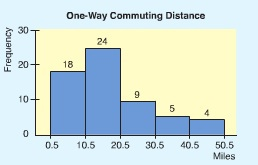
\includegraphics[scale=0.75]{WS3_Commute.jpg}
\end{center}

	\begin{enumerate}
	\item We have no idea how the 24 values within the class boundaries 10.5-20.5 are distributed.  However, if we wanted to estimate their approximate value to compute the mean, what value would be the best choice to represent those 24 values?
	
	{\answer{A reasonable estimate would be to use the midpoint of each class.  So, in particular, for the 24 values between 10.5 and 20.5, use the value 15.5 to represent them.}} 
	
	\item Using this idea, estimate the mean commuting distance for the employees that answered the survey.

	{\answer{With $L_1 = \textnormal{ midpoints of distance intervals}$ and $L_2 = \textnormal{ frequencies}$,
	1-Var Stats $L_1$, $L_2$ yields $\bar{x} = 17.67$.}} 

	\end{enumerate}

%Section 3.1 #10
\item Consider two data sets.
\begin{center} 
Set A: $n=5$, $\bar{x} =10$ \hspace{2.0in} Set B: $n=50$; $\bar{x}=10$ 
\end{center}
	\begin{enumerate}
	\item Suppose the number 20 is included as an additional data value in Set A.  Compute $\bar{x}$ for the new data set. 
	
	{\answer{Now Set A has $n=6$ data values.  To determine the new mean, we must first determine what the sum of the original 5 values must have been.  That is, for the original 5 data values $\sum x = n\bar{x} = 5(10) = 50$.  Including the new value, the sum of all data values in the set is $50 + 20$ and the mean is $\bar{x} = \frac{70}{6} = 11.67$. }} 
	
	\item Suppose the number 20 is included as an additional data value in Set B.  Compute $\bar{x}$ for the new data set. 
	
	{\answer{Now Set B has $n=51$ data values.  To determine the new mean, we must first determine what the sum of the original 50 values must have been.  That is, for the original 50 data values $\sum x = n\bar{x} = 50(10) = 500$.  Including the new value, the sum of all data values in the set is $500 + 20$ and the mean is $\bar{x} = \frac{520}{51} = 10.20$. }} 
	
	\item Why did the addition of the number to each set change the mean more in one case than in the other?
	
	{\answer{Because Set B is a larger sized set, the addition of that one new value has less impact on the mean than in the smaller sized Set A.}} 
	
	\end{enumerate}

\newpage

\item A VERY common question from students towards the end of the semester is ``What score do I need on the final exam to get a (fill in the blank) in the class?" For this class, this requires working with a weighted average.  So, let's try this exercise for a sample student in this class. \\
Here are the scores for the student going into the final exam: \\
15\% - Midterm 1 (out of 100) - 77; \\ 
15\% - Midterm 2 (out of 100) - 81; \\
10\% - Participation (average out of 100) - 100; \\
10\% - Reading Quizzes (average out of 100) - 98; \\
10\% - Chapter Reviews (each out of 100) - 100, 98, 87, 100, 92, 90, 83, 100, 100, 82 ; \\
10\% - Projects (each out of 100) - 82, 76; \\
10\% - Quizzes (each out of 10) - 5, 8, 7.5, 10, 8, 6, 8, 10, 7, 6.5, 7, 6; (where the lowest two will be dropped)

	\begin{enumerate}
	\item What is the weighted average for this student for all scores except the final? 
	
	{\answer{After dropping the lowest two quiz scores (5 and one 6), the weighted average is $$\frac{0.77*0.15 + 0.81*0.15 + 1.00*0.1 + 0.98*0.10 + 0.932*0.10 + 0.79*0.10+ 0.78*0.10}{0.15+0.15+0.1+0.10+0.10+0.10+0.10} = 0.8565.$$}} 
	
	\item What is the minimum score that the student can earn on the final exam to earn a grade of `B-' or better?  (Assume that a student must earn an 80\% or higher overall (NO rounding up) in the course to earn an `B-'.)

	{\answer{Then, if we let $E$ represent the final exam, the student needs $$\frac{0.8565*0.80+E*0.20}{0.80+0.20}=0.80 \textnormal{ or equivalently } E = \frac{0.80-0.8565*0.80}{0.20} = 0.574.$$  So, a 57.4\% on the final will result in a 'B-' overall.}} 

	\item (Challenge!) What is the minimum score that the student can earn on the final exam to earn a grade of `A-' or better?  (Assume that a student must earn an 90\% or higher overall (NO rounding up) in the course to earn an `A-'.) Don't forget about the midterm replacement policy!
	
	{\answer{If the final exam is greater than 77\%, the final exam will replace the midterm 1 score, as it is the lower of the two. Note the weighted average of all scores, except the final and midterm 1 is
	$$\frac{0.81*0.15 + 1.00*0.1 + 0.98*0.10 + 0.932*0.10 + 0.79*0.10+ 0.78*0.10}{0.15+0.1+0.10+0.10+0.10+0.10} \approx 0.8765.$$
	So the student needs 
	$$\frac{0.8765*0.65 + E*.35}{0.65+0.35} = 0.9 \Rightarrow E=\frac{0.9-0.8765*0.65}{0.35} \approx 0.9437,$$ or a 94.37\%.}}
	
	\end{enumerate}

\vfill

\end{enumerate}

\vfill

\end{document}

